\documentclass[11pt, sans, handout]{beamer}

\usepackage[utf8]{inputenc} 
\usepackage[T1]{fontenc}
\usepackage{lmodern}
\usepackage{graphicx}
\usepackage[french]{babel}
\usepackage[many]{tcolorbox}

\newtcolorbox{RDB}[2][]{%attach boxed title to top center
               = {yshift=-8pt},
  colback      = blue!5!white,
  colframe     = blue!75!black,
  fonttitle    = \bfseries,
  colbacktitle = blue!85!black,
  title        = #2,#1,
  enhanced,
}

\usetheme{Copenhagen}

\addtobeamertemplate{footline}{\insertframenumber/\inserttotalframenumber}


\begin{document}
\title{Titre}
\maketitle

\frame{
   \frametitle{Sommaire}
   \tableofcontents[currentsubsection,sectionstyle=show/shaded,subsectionstyle=show/shaded/hide]
}

\frame{
	\frametitle{Rappel théorique}
	\framesubtitle{Base de données relationnelle}
	Dans une base de données relationelle, les données sont organisées en tables. Les colonnes de ces tables sont appelées des attributs et les lignes sont appelées des tuples.\\
	\begin{center}
	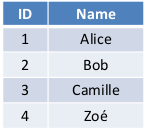
\includegraphics[scale=0.62]{resources/BDR1.png}
	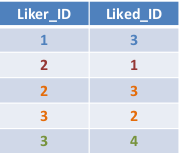
\includegraphics[scale=0.62]{resources/BDR2.png}
	\end{center}
	Les tables d'une BDR respectent des contraintes et des clés.\\
}

\frame{
	\frametitle{Rappel théorique}
	\framesubtitle{Base de données en graphe}
	Dans une base de données en graphe, les données sont contenues dans des noeuds, et les relations entre les données sont décrite par les arcs reliant ces noeuds. A chaque tupe des tables d'une BDR correspond un noeud en BDG. La base de donnée prend la forme d'un graphe orienté.
	\begin{center}
	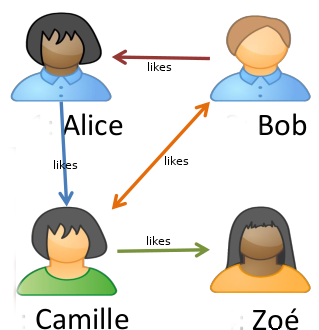
\includegraphics[scale=1.75]{resources/BDG1.png}
	\end{center}
}

\frame{
	\frametitle{Comparaison des modèles}
	\framesubtitle{Efficacité lors de la séléction}
	Maintenant que nous avons nos données stockées selon les deux modèles, effectuons une requête.
	Commencons par une requête simple :
	\emph{Qui est-ce que Bob aime ?}
}
	\frametitle{Comparaison des modèles}
	\framesubtitle{Efficacité lors de la séléction}
	
\frame{
	\frametitle{Comparaison des modèles}
	\framesubtitle{Efficacité lors de la séléction}
	Dans notre base de données relationnelle :\\
	\begin{itemize}
		\item Rechercher dans la table (ID, name) Bob, pour connaitre son ID.
		\item Rechercher dans la table (liker\_ID, liked\_ID) toutes les occurence de l'ID de Bob.
	\end{itemize}
	\begin{center}
		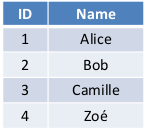
\includegraphics[scale=0.62]{resources/BDR1.png}
		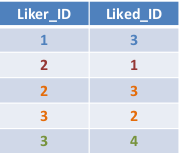
\includegraphics[scale=0.62]{resources/BDR2.png}
	\end{center}
}

\frame{
	\frametitle{Comparaison des modèles}
	\framesubtitle{Efficacité lors de la séléction}
	Dans notre base de données en graphe :\\
	\begin{itemize}
		\item Trouver Bob.
		\item Les arcs "liked" partant de Bob nous donne immédiatement l'information recherchée.
	\end{itemize}
	\begin{center}
	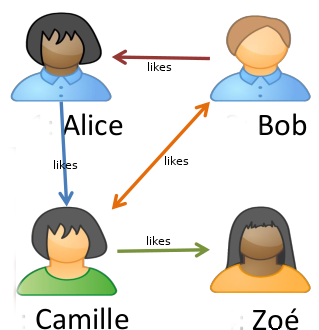
\includegraphics[scale=1.75]{resources/BDG1.png}
	\end{center}
}

\frame{
	\frametitle{Comparaison des modèles}
	\framesubtitle{Efficacité lors de la séléction}
	Intéressons nous maintenant à une requête plus compliquée sur une autre base de données.\\
	\emph{Quel est ce film parlant de sous-marins dans lequel joue l'acteur qui était dans un autre film aux cotés de l'acteur principal de "Gone With the Wind" ?}
}

\frame{
	\frametitle{Comparaison des modèles}
	\framesubtitle{Efficacité lors de la séléction}
	Dans notre base de données relationnelle :\\
	\begin{itemize}
		\item Trouver les acteurs de "Gone With the Wind".
		\item Trouver tous les films dans lesquels ces acteurs ont joués.
		\item Trouver tous les acteurs ayant joués dans ces films et n'étant pas l'acteur principal de "Gone With the Wind".
		\item Trouver tous les films dans lesquels chacuns de ces acteurs ont joués.
		\item Finalement, rechercher le mot "sous-marin" dans la description de ceux-ci.
	\end{itemize}
}

\frame{
	\frametitle{Comparaison des modèles}
	\framesubtitle{Efficacité lors de la séléction}
	Dans notre base de données en graphe :\\
	\begin{itemize}
		\item Trouver le noeud "Gone With the Wild".
		\item Suivre le lien "a comme acteur principal" pour arriver a Clark Gable.
		\item Suivre les liens "a joué dans" en partant de celui-ci.
		\item Suivre les liens "a pour acteur" en partant des films ainsi atteints.
		\item Suivre les liens "a joué dans" en partant de ceux-ci.
		\item Examiner les noeuds atteints à la recherche du mot "sous-marin".
	\end{itemize}
	Nous n'avons fait que suivre des liens, aucune recherche n'a été effectuée.
}


\frame{
	\frametitle{A venir}
	RDB\\
-Lourd en execution avec les jointures (mutliples recherches)\\
-Lourd écriture + connaissance obligée\\
-Moins flexible, demande de re design les table si on veut ajouter un élément ponctuel\\

-Mieux pour des recherche au sein d'une table donnée, ou pour appliquer une transformation à chaque ligne d'une table\\

-Design plus mature, plus étudié\\
-Existent déjà partout. Ce n'est pas un avantage mais c'est un désavantage pour GDB: on ne peut pas nier que les gros changements sont un désavantage, même si l'autre modèle est jugé intrinsèquement mieux\\
	=> utilisation mixée des deux modèles.
}
\end{document}